\chapter{Variational Methods}

In this lecture, we investigate use of \textit{variational principles} in the 
context of nuclear engineering.  An entire course could be devoted to this 
subject; here, we focus on the same two quantities analyzed in 
Lecture \ref{lec:adjoint}, namely the reaction rate for a fixed source problem 
and the eigenvalue of an eigenvalue problem.  We demonstrate that variational 
principles can be used to estimate these quantities using approximate fluxes. 
We finish by showing how our first order perturbation theory can be derived 
directly from variational principles.

%------------------------------------------------------------------------------%
\section*{Variational Principles, Functionals, and Stationary Points}

A variational principle casts a particular function, usually a problem's 
solution, as the stationary point of some \textit{functional}. Often, the 
functional itself is called the variational principle.  A functional is 
simply a function that takes another function as its argument and returns 
a scalar as its value.  Consider a function $f(x) = Ax + B$.  A possible 
functional would be $F[f(x)] = \int_{x_1}^{x_2} f(x)dx$, which certainly 
yields a scalar value.  Typically, the value of the functional represents 
a quantity of interest, which in transport applications is often a 
reaction rate.

We see that functionals are quite like functions; how exactly then do we 
define a \textit{stationary point}, and what does it mean in the context 
of a variational principle?  Recall from elementary calculus that a stationary 
point is the value of the independent variables such that the function reaches 
a local extremum (or saddle-point), i.e. the function's derivative (or 
gradient) vanishes.  The same idea applies to functionals.  Defining 
the ``weak derivative'' of $F$ at a point $f(x)$ in the direction $g(x)$ as
\begin{equation}
 \delta F[f,g] = \lim_{\epsilon \to 0} 
                 \frac{ F[f+\epsilon g] - F[f] }{\epsilon} \, ,
\end{equation}
the \textit{first variation} of $F$ is defined 
\begin{equation}
 \delta F[f,g] = \left ( \frac{d}{d\epsilon} F[f+\epsilon g] \right ) 
                 \Bigg |_{\epsilon = 0} \, ,
\end{equation}
for arbitrary $g$.  When $\delta F[\tilde{f},g] = 0$ for all $g$, $\tilde{f}$ 
is called a \textit{stationary point} of $F$, and the expression
\begin{equation}
 \delta F[\tilde{f},g] = 0 \, ,  \, \, \, \, \, \, \forall g 
\end{equation}
defines the variational principle for $\tilde{f}$.  For $F[f]$ that represents 
a quantity of interest, $F[\tilde{f}]$ represents the true value for that 
quantity.  Moreover, very near the stationary point, $\delta F \to 0$ by 
construction, and the errors in $F$ (and hence the quantity of interest) are 
second order, which gives rise to the utility of variational approximations.

%------------------------------------------------------------------------------%
\section*{A Simple, Illustrative Example}

It is easiest to understand these ideas through a simple example (unrelated 
to nuclear engineering).  Suppose we wish to find the curve giving us the 
shortest difference between two points in a plane  Of course, this is 
intuitive: the solution should be a line.  We show this using variational 
techniques.  

Let the curve be $f(x)$. From any calculus book, we know the differential arc 
length is then
\begin{equation}
 dl = \sqrt{ dx^2 + df^2 } = \sqrt{1 + (f')^2} \, .
\end{equation}
We take as our functional the arc length,
\begin{equation}
 F[f] = \int^{x_2}_{x_1} \sqrt{1 + (f')^2} dx \, ,
\end{equation}
where ($x_1$, $y_1$) and ($x_2$, $y_2$) are the points of interest, as 
illustrated in Figure \ref{fig:shortest_path}.

\begin{figure}[ht] 
    \centering
    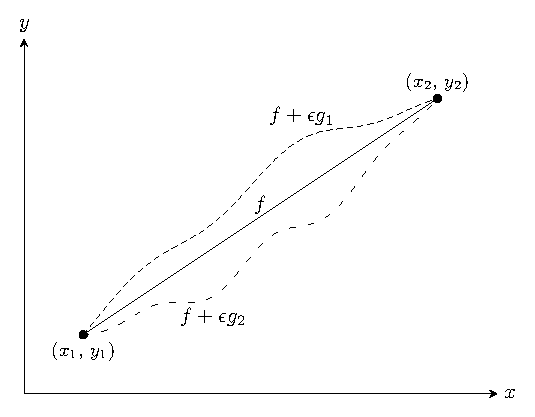
\includegraphics[keepaspectratio, width = 4.0 in]{images/shortest_path}
    \caption{The shortest path between two points ($x_1$, $y_1$) and 
            ($x_2$, $y_2$) is indicated by the solid curve $f$.  Two possible
            curves for arbitrary $g$ are also given.}
    \label{fig:shortest_path}
\end{figure} 

Taking the first variation of $F$,
\begin{equation}
\begin{split}
\delta F[f,g] &= \left ( \frac{d}{d\epsilon}\int^{x_2}_{x_1} 
                         \sqrt{1 + (f'(x)+\epsilon g'(x))^2} dx \right ) 
                 \Bigg |_{\epsilon=0} \\
              &= \left ( \int^{x_2}_{x_1} 
                         \frac{(f'(x)+\epsilon g'(x))g'(x)}
                              {\sqrt{1 + (f'(x)+\epsilon g'(x))^2}} \right ) 
                 \Bigg |_{\epsilon=0} \\
              &= \int^{x_2}_{x_1} \frac{f'(x)g'(x)dx}{\sqrt{1 + (f'(x))^2}} \, ,
\end{split}
\end{equation}
we find that the arc length is minimized when
\begin{equation}
 \delta F[y,g] =
   \int^{x_2}_{x_1}\frac{f'(x)g'(x)}{\sqrt{1 + (f'(x))^2}} = 0 \, .
 \label{eq:exampleprinciple}
\end{equation}
In this form, we can't say anything about $f$ or $g$.  Instead, we use 
integration by parts to go from $f'$ and $g'$ to $f''$ and $g$, and
Eq. \ref{eq:exampleprinciple} becomes
\begin{equation}
 \delta F[f,g] =
   \left [ \frac{f'(x)g(x)}{\sqrt{1 + (f'(x))^2}} \right ]^{x_2}_{x_1} - 
   \int^{x_2}_{x_1} \frac{f''(x)g(x)dx}{(1 + (f'(x))^2)^{\frac{3}{2}}} = 0\, .
 \label{eq:exampleprinciple2}
\end{equation}
While $g(x)$ is arbitrary \textit{between} $x_1$ and $x_2$, we must have 
$g(x_1) = g(x_2) = 0$ to that $f(x_1) = y_1$ and $f(x_2) = y_2$.  Thus, the 
first term of Eq. \ref{eq:exampleprinciple2} vanishes. 
By inspection, the second term vanishes for 
arbitrary $g$ only if $f'' = 0$.  This relation is known as 
the \textit{Euler equation}\footnote{In general, setting the first variation 
to zero gives rise to a set of partial differential equations collectively 
known as the Euler equations.}.  Of course, to satisfy $f''=0$ requires 
our solution to be of the form $Ax+B$, as expected.

%------------------------------------------------------------------------------%
\section*{A Variational Principle for Fixed Source Problems}

Suppose we are interested in a linear functional of the flux, such 
as $G_{\text{fs}}[\psi] = \langle \psi, \Sigma_d \rangle$, a reaction rate. 
An appropriate variational principle is represented by 
the \textit{generalized Roussopoulos functional}
\begin{equation}
 F_{\text{fs}} [\psi,\psi^*] = 
   G_{\text{fs}}[\psi] + \langle \psi^*, (Q-L\psi) \rangle \, .
\end{equation}
Note, $\delta F_{\text{fs}}[\psi,\psi^*] = 0$ is a variational principle 
for $G_{\text{fs}}$ if the corresponding solution $\psi$ 
yields $F_{\text{fs}}[\psi,\psi^*] = G_{\text{fs}}[\psi]$.  We see this is 
so when the second term of $F$ vanishes when $\psi$ solves $L\psi = Q$, i.e. 
when $\psi$ is the solution to the transport equation.

To determine the variational principle, we take the first variation 
of $F_{\text{fs}}$,
\begin{equation}
 \begin{split}
  \delta F_{\text{fs}} & [\phi,\phi^*] \\
   &= \left ( \frac{d}{d\epsilon} 
            \left ( \langle (\phi+\epsilon \delta \phi) \Sigma_d \rangle + 
                    \langle (\phi^* + \epsilon \delta \phi^*), 
                            (Q-L(\phi+\epsilon \delta \phi)) \rangle 
            \right ) 
    \right ) \Bigg|_{\epsilon=0} \\
   &= \langle \delta \phi, \Sigma_d \rangle - 
      \langle \phi^*,L \delta \phi \rangle + 
      \langle \delta \phi^*, Q \rangle - 
      \langle \delta \phi^*, L \phi \rangle +
      \mathcal{O}(\epsilon^2) \, .
 \end{split}
\end{equation}
Noting 
$\langle \phi^*,L\delta \phi \rangle = \langle L^* \phi^*,\delta \phi \rangle$, 
we have for our principle 
\begin{equation}
 0 = \langle \delta \phi, (\Sigma_d - L^* \phi^*) \rangle + 
     \langle \delta \phi^*, (Q-L\phi) \rangle \, ,
\end{equation}
which is satisfied when $L\phi = Q$ and $L^* \phi^* = \Sigma_d$.  These are 
the corresponding Euler equations, and we see they are just the original 
forward and adjoint transport equations.

The importance of this variational principle (and others in general) is that 
it gives us an estimate for $G_{\text{fs}}$ accurate to second order for 
approximate fluxes $\phi$ and $\phi^*$.  To demonstrate this, suppose the 
true solutions to the Euler equations are $\psi$ and $\psi^*$.  
Let $\phi = \psi + \delta \psi$ and $\phi^* = \psi^* + \delta \psi^*$.  
We subsitute these expressions into $F$ and find
\begin{equation}
 \begin{split}
    F_{\text{fs}} [\phi,\phi^*] &= 
      \langle \Sigma_d, (\psi+\delta \psi) \rangle + 
      \langle (\psi^*+\delta \psi^*),(Q-L(\psi+\delta \psi^*) \rangle \\
    &= \langle \Sigma_d,\psi \rangle + 
       \langle \Sigma_d, \delta \psi \rangle + 
       \langle \psi^*,Q \rangle + 
       \langle \delta \psi,Q \rangle  \\ 
    &- \langle \psi^*, L\psi \rangle - 
       \langle \psi^*, L\delta \psi \rangle - 
       \langle \delta \psi^*, L\psi \rangle - 
       \langle \delta \psi^*, L\delta \psi \rangle \\
    &= \langle \Sigma_d, \psi \rangle - 
       \langle \delta \psi^*, L\delta \psi \rangle \\
    &= G_{\text{fs}}[\psi] + \mathcal{O}(\delta^2) \, .
 \end{split}
 \label{eq:secondorderfs}
\end{equation}
Hence, $F$ provides a first order accurate (i.e. good through first order) 
estimate of the reaction rate given approximate forward and adjoint fluxes.

\section*{A Variational Principle for Eigenvalue Problems}

For eigenvalue problems, an appropriate functional is 
the \textit{Rayleigh quotient}
\begin{equation}
 F_{\text{ev}}[\psi,\psi^*] = 
   \frac{\langle \psi^*,L\psi \rangle}{ \langle \psi^*, F \psi \rangle } \, .
 \label{eq:rayleigh}
\end{equation}
Here, the quantity of interest is $G_{\text{ev}} = \lambda$, and, unlike the 
fixed source case, we have $G_{\text{ev}} = F_{\text{ev}}$.  You should show 
that $F_{\text{ev}}$ is in fact a valid expression for $\lambda$.  The 
associated Euler equations are just the forward and adjoint eigenvalue 
equations, which can be shown by setting the first variation 
of $F_{\text{ev}}$ to zero, an exercise left to the reader.
For approximate fluxes $\phi$ and $\phi$
\begin{equation}
 F_{\text{ev}}[\phi,\phi^*] = \lambda + \mathcal{O}(\delta^2) \, ,
\end{equation}
the proof of which is also left as an exercise.

\section*{Perturbation Theory from Variational Principles}

In general, it is possible to find first order perturbation estimates using 
the expression
\begin{equation}
 \delta = \bar{F}[\psi,\psi^*] - F[\psi,\psi^*] \, ,
 \label{eq:pertfromvar}
\end{equation}
where $F$ is the appropriate functional with nominal operators 
and $\bar{F}$ is the function evaluated with perturbed operators.  It must 
be stressed that $\psi$ and $\psi^*$ are assumed to be the exact fluxes for 
the unperturbed problem.

As an example, we re-derive the first order perturbation to a detector 
response.  Suppose the perturbations to our system 
include $L+\delta L$, $Q+\delta Q$, 
and $\Sigma_d + \delta \Sigma_d$.  Then Eq. \ref{eq:pertfromvar}  gives
\begin{equation}
\begin{split}
 \delta_{\text{fs}} &= \bar{F}[\psi,\psi^*] - F[\psi,\psi^*] \\
        &= \langle \psi, (\Sigma_d+\delta \Sigma_d) \rangle + 
           \langle \psi^*,(Q+\delta Q-(L+\delta L)\psi ) \rangle - 
           \langle \psi, \delta \Sigma_d \rangle \\
        &= \langle \psi,\delta \Sigma_d \rangle + 
           \langle \psi^* , \delta Q \rangle - 
           \langle \psi^*,\delta L \psi \rangle \, .
\end{split}
\label{eq:fixedpertvar}
\end{equation}
The last line is equivalent to Eq. \ref{eq:fixedpertresp} with the addition 
of the first term, which explicitly accounts for changes in the detector 
response function.

Eq. \ref{eq:pertfromvar} can also be applied to the Rayleigh quotient, 
yielding Eq. \ref{eq:eigenpertresp}, proof of which is left 
as an exercise.

%------------------------------------------------------------------------------%
\section*{Further Reading}

Most of the material presented here is contained in Chapter 7 of 
Duderstadt and Martin \cite{duderstadt1976tt}  in addition to Chapter 1 
of Stacey \cite{stacey1974vmn}.  The former contains several examples 
and a variational derivation of the diffusion equation.  The reader is 
also encouraged to look up Pomraning's large body of work on variational 
methods\footnote{It is worth noting that Stacey and Pomraning, both with 
prolific work in variational methods, did their graduate work in 
this department.}.

%------------------------------------------------------------------------------%
\begin{exercises}

  %----------------------------------------------------------------------------%
  \item \textbf{Second Order Accuracy}. 
    Show that the Roussopoulos functional $F[\phi,\phi^*]$ gives a second 
    order accurate value for $\langle \psi,\Sigma_d \rangle$ when $\phi$ 
    and $\phi^*$ are approximate values of $\psi$ and $\psi^*$, i.e. 
    prove Eq. \ref{eq:secondorderfs}.

  %----------------------------------------------------------------------------%
  \item \textbf{Fixed Source Perturbation}. 
    Prove Eq. \ref{eq:fixedpertvar}.
 
  %----------------------------------------------------------------------------%
  \item \textbf{Rayleigh Quotient}. 
    \begin{enumerate}[a.]
      \item Take the first variation of the Rayleigh quotient with respect to 
            the forward and adjoint fluxes and show the stationarity conditions 
            are just the forward and adjoint eigenvalue problems. 
      \item Demonstrate that the Rayleigh quotient is a second order 
            estimator for $\lambda$.
    \end{enumerate}

  %----------------------------------------------------------------------------%
  \item \textbf{Losses-to-Gains}. 
    Directly from the eigenvalue equation, we find 
    \begin{equation*}
      \lambda = (L\psi)/(F\psi) \, ,
    \end{equation*}
    a compact way to define losses-to-gains.  
    \begin{enumerate}[a.]
      \item Show why this is not a variational principle for $\lambda$.
      \item Consider again Eq. \ref{eq:rayleigh}.  How does the adjoint change 
            the physical interpretation of gains-to-losses?
    \end{enumerate}

  %----------------------------------------------------------------------------%
  \item  \textbf{Eigenvalue Perturbation}. 
    Prove that $\bar{F}_R[\psi,\psi^+]-F_R[\psi,\psi^+]$ yields the first 
    order perturbation estimate for $\delta \lambda$ given 
    by Eq. \ref{eq:eigenpertresp}.

  %----------------------------------------------------------------------------%
  \item  \textbf{Applying Roussopoulos}. 
    Consider a 1-d, 1-speed diffusion problem in a slab of 
    width $2a$, $\Sigma_a = 0.022$, and $D = 0.14$. 
    \begin{enumerate}[a.]
      \item Solve for the exact scalar flux $\phi(x)$, using the 
            conditions $\phi(\pm a)=0$, and
            assuming a uniform source $Q(x) = 1$ and $a=1$.
      \item Compute the total absorption rate in the slab.
      \item Now, approximate the solution as 
            $\tilde{\phi}(x) = Ax^2 + Bx +C$ with the same maximum 
            and the same boundary conditions.  Compute the absorption rate  
            using $\tilde{\phi}(x)$.
      \item Finally, recalling the 1-d, 1-speed diffusion equation is 
            self-adjoint, use the Roussopoulos principle to compute the 
            absorption rate.  What can you conclude? 
    \end{enumerate}

  %----------------------------------------------------------------------------%
  \item \textbf{More Roussopoulos}. 
    For the same problem, estimate the total absorption rate if something 
    causes $\Sigma_a = 1.1$.  Be careful to consider the impact of the change 
    in $\Sigma_a$ on both $\Sigma_d$ and $L$.

  %----------------------------------------------------------------------------%
  \item \textbf{Approximating Escape from a Slab}. 
    Recall the escape probability $P_{\text{esc}}$ for a homogeneous 1-d slab, 
    the subject of 
    Chapter \ref{lec:analytical}, Problem \ref{itm:escapeprobability}.  
    Here, consider a discrete ordinates approximation using the 
    two point Gauss-Legendre quadrature and Mark boundary conditions
    for a 10 cm slab with $\Sigma_t = 10$ [1/cm].
    \begin{enumerate}[a.]
      \item Solve for $P_{\text{esc}}$ directly using the S$_{\text{2}}$ 
            approximation.
      \item Use a variational principle to improve 
            your estimate of $P_{\text{esc}}$. 
      \item Compare both values to the exact value.
    \end{enumerate}

\end{exercises}
